% ----------------------------------------------------------------------------
% main.tex — DS 299 Capstone, IEEE conference format
%
% Submitted to CODASSCA 2026, Track 4 (AI / Neural Networks / Deep Learning)
% Format: IEEEtran [conference], 6 pages (full paper)
% Submission: easychair.org/conferences/?conf=codassca2026, deadline 2026-05-15
%
% Class option `conference` produces two-column conference-style output.
% Swap to `journal` (or remove the option) to get IEEE Transactions style.
% ----------------------------------------------------------------------------

\documentclass[conference]{IEEEtran}

% --- Packages ---------------------------------------------------------------
\usepackage{amsmath}
\usepackage{amssymb}
\usepackage{graphicx}
\usepackage{booktabs}
\usepackage[hidelinks]{hyperref}

% Optional polish pkgs (not in current TinyTeX install — re-enable once
% available: `tlmgr install microtype siunitx cleveref`):
% \usepackage{microtype}
% \usepackage{siunitx}
% \usepackage[capitalize]{cleveref}

% --- Figure path ------------------------------------------------------------
\graphicspath{{figures/}}

% --- Title and authors ------------------------------------------------------
\title{Beyond Right Answers: External-Judge Validation of LLM Bayesian Reasoning}

\author{%
  \IEEEauthorblockN{Albert Simonyan}
  \IEEEauthorblockA{%
    \textit{B.S. Data Science, Akian College of Science and Engineering} \\
    \textit{American University of Armenia} \\
    Yerevan, Armenia \\
    albert.simonyan.w@gmail.com}
  \and
  \IEEEauthorblockN{[Advisor Name --- TODO]}
  \IEEEauthorblockA{%
    \textit{Akian College of Science and Engineering} \\
    \textit{American University of Armenia} \\
    Yerevan, Armenia \\
    {}[advisor email --- TODO]}%
}

% ----------------------------------------------------------------------------
\begin{document}

\maketitle

% --- Section: Abstract ---

\begin{abstract}
Failure modes are disguised on accuracy-only leaderboards, and the
disguise matters when LLMs are used to solve statistical problems.
Five frontier models (Claude Sonnet 4.5, GPT-4.1, Gemini 2.5 Flash,
DeepSeek-Chat, Mistral Large) are benchmarked against 171 Bayesian
and inferential tasks across 38 types with 473 perturbations on
three axes: rephrase, semantic, and numerical. Each response is
scored twice, by a deterministic keyword rubric and by an
out-of-family judge (Llama 3.3 70B Turbo, served via Together AI)
on assumption-compliance and reasoning quality. The rankings
disagree. GPT-4.1 places last on accuracy (0.621) but first on
robustness (0.9996). Claude leads accuracy (0.683) and binary-pass
calibration (ECE 0.0334), yet drops to fourth on robustness
(0.9565). 44.3\% of responses do not mention the assumptions the
derivation depends on, and assumption violation drives 47\% of
judge-classified failures. The keyword rubric and the judge agree
only moderately on assumption-compliance (Spearman 0.602) and
barely at all on the two other judged dimensions. A single-number
leaderboard is the wrong instrument here: which model wins depends
on the metric.
\end{abstract}

\begin{IEEEkeywords}
LLMs, Bayes' theorem, calibration, perturbation robustness,
expected calibration error, LLM-as-judge, benchmark
\end{IEEEkeywords}

% --- Section: Introduction ---
% Drafted Phase 5 — values pulled from cleanup/04_phase5_data_pulled.md
% Target: ~600–800 words.

\section{Introduction}
\label{sec:intro}

Many users of large language models pick a model by reading the top
of a leaderboard. For statistical reasoning that habit is risky.
Benchmarks such as StatEval~\cite{lu2025stateval},
MathEval~\cite{liu2025matheval}, the human-comparison study of
Nagarkar et al.~\cite{nagarkar2026canllm}, and ad-hoc evaluations on
Bayesian tasks~\cite{longjohn2025bayesian} report accuracy alone.
But accuracy fuses three properties that a downstream user actually
cares about separately: whether the model lands on the right number,
whether it does so when the prompt is reworded or the numbers are
swapped, and whether its stated confidence tracks its empirical
correctness. When those three disagree, a single accuracy column is
misleading.

We make the disagreement concrete on 171 Bayesian and inferential
tasks. Five frontier LLMs are scored on accuracy, robustness, and
calibration; the rank orders differ. Two patterns are doing most of
the work. GPT-4.1, last on accuracy (0.621), is first on robustness
(0.9996); its base and perturbation pass rates are within 0.0003 of
each other. Claude leads accuracy (0.683) and binary-pass calibration
(ECE 0.0334) but drops to fourth on robustness (0.9565), losing three
percentage points between base and perturbed prompts. A consumer who
reads only the accuracy column never sees either pattern, and the
deployment advice each one implies is different. Separately, 44.3\%
of responses fail to state the statistical assumptions the derivation
requires, even when the final number is correct, and assumption
violation is the dominant failure mode at 47\% of judge-classified
failures. Du et al.~\cite{du2025icecream} report the same blindness
in causal reasoning.

The methodological gap behind the headline also bears naming. Most
LLM-statistics evaluations rely on a keyword rubric, a single judge,
or both, and both have known biases. Keyword rubrics confuse surface
form with substance: the word ``assume'' in a response is not the
same thing as actually stating an assumption. Single-judge protocols
suffer self-preference bias and design-choice sensitivity, as
documented by Yamauchi et al.~\cite{park2025judge} and Feuer et
al.~\cite{judgment2025noise}. We score each response twice, once with
a deterministic keyword rubric in the live runner and once with an
external, out-of-family judge: Llama 3.3 70B Turbo via Together AI,
not one of the five benchmarked models. The two views disagree where
it matters. They agree only moderately on assumption-compliance
(Spearman 0.602) and barely at all on method structure and reasoning
quality. The keyword rubric also passes assumptions more leniently
than the judge (71.1\% vs 55.7\%), which is why keyword-only
protocols read Bayesian competence higher than it is.

Our contributions are:
\begin{enumerate}
  \item A benchmark of 171 Bayesian and inferential tasks (136
        closed-form conjugate models and 35 computational Bayesian
        methods covering Gibbs, Metropolis-Hastings, HMC, RJMCMC,
        hierarchical, VB, and ABC) with 473 perturbations along
        three axes (rephrase, semantic, numerical) that touch all
        38 task types.
  \item An external-judge protocol using an out-of-family open-weights
        model (Llama 3.3 70B Turbo) for assumption-compliance and
        reasoning quality. Keyword-rubric vs judge agreement is
        reported per dimension (Spearman 0.602 on
        assumption-compliance, much lower elsewhere). The split
        between what a rubric can see and what a judge can see is
        itself a finding.
  \item Empirical evidence that accuracy, robustness, and calibration
        rankings of the same five LLMs disagree non-trivially. The
        two flagship divergences are a 5-to-1 inversion between
        accuracy and robustness (GPT-4.1) and a 1, 1, 4 pattern for
        the accuracy-and-calibration leader (Claude). Neither shows
        up on a single-metric leaderboard.
  \item An open audit trail. NMACR scoring weights (A=0.30, R=0.25,
        M=0.20, C=0.15, N=0.10), aggregation choices, and tolerance
        thresholds are all documented and tied to the papers that
        motivated them.
\end{enumerate}

Section~\ref{sec:related} reviews statistical-reasoning benchmarks,
the calibration literature~\cite{guo2017calibration}, and
LLM-as-judge work~\cite{zheng2023judge,park2025judge,judgment2025noise}.
Section~\ref{sec:methodology} covers the task suite, perturbations,
judge protocol, and experimental setup. Section~\ref{sec:results}
presents the three rankings. Section~\ref{sec:discussion} argues
the divergence is not noise. Section~\ref{sec:conclusion} closes
with threats to validity and future work.

% --- Section: Related Work ---
% Drafted Phase 6 — values pulled from cleanup/04_phase5_data_pulled.md
% Target: ~400 words.

\section{Literature Review}
\label{sec:related}

\textbf{LLM benchmarks for quantitative reasoning.}
StatEval~\cite{lu2025stateval} catalogues 13{,}817 problems across
descriptive statistics, probability, inference, and regression,
scored mainly by answer correctness.
MathEval~\cite{liu2025matheval} compares 23 LLMs across 19
mathematical-reasoning datasets, again on accuracy. Nagarkar et
al.~\cite{nagarkar2026canllm} compare LLMs to human respondents on
statistical tasks. All three report how often the model lands on
the right number, but none asks whether the reasoning that produced
the number is well-formed or stable under perturbation.

\textbf{Bayesian-reasoning evaluation.} Longjohn et
al.~\cite{longjohn2025bayesian} propose a Bayesian framework for
aggregating benchmark results probabilistically, not for evaluating
Bayesian reasoning itself. Du et al.~\cite{du2025icecream} document
assumption-blindness in causal reasoning: LLMs produce
``convincing yet misleading'' answers without articulating the
assumptions those answers depend on. The 44.3\% missing-assumption
rate we report extends the same pattern to inferential statistics.

\textbf{Calibration.} Guo et al.~\cite{guo2017calibration}
introduced Expected Calibration Error (ECE) and showed that modern
neural networks are systematically miscalibrated despite high
accuracy. ECE is well-studied for classifiers; its application to
free-form LLM reasoning is recent and less settled. FermiEval and
related work~\cite{fermieval2025,multianswer2026,nagarkar2026canllm}
adapt calibration to natural-language outputs, but typically on a
single dimension. We report binary-pass ECE and a per-NMACR-dimension
ECE.

\textbf{LLM-as-judge.} Zheng et al.~\cite{zheng2023judge}
popularised LLM-as-judge with MT-Bench, showing that strong LLMs
can substitute for human raters on open-ended tasks. Follow-up work
documents design-choice sensitivity and self-preference
bias~\cite{park2025judge,judgment2025noise}. Brittlebench and
ReasonBench~\cite{brittlebench2026,reasonbench2025} document prompt
sensitivity and reasoning instability under perturbation. Our
protocol constrains the judge to a single dimension
(assumption-compliance) and uses an out-of-family open-weights
model (Llama 3.3 70B Turbo). Both choices address failure modes
that Feuer et al.~\cite{judgment2025noise} document.

Across these threads, evaluation usually collapses to one accuracy
or pass-rate number. We pull the three threads together into a
tri-axis ranking and report the disagreement across the same five
LLMs on the same task suite.

\textbf{Positioning.} Prior work treats accuracy, robustness, and
calibration as separable evaluation concerns and tackles them in
isolation. Quantitative-reasoning benchmarks measure accuracy at
scale but rarely report robustness or
calibration~\cite{lu2025stateval,liu2025matheval,nagarkar2026canllm}.
Calibration studies operate on classification or short-answer
formats, not on the free-form numerical and prose responses typical
of Bayesian reasoning~\cite{guo2017calibration}. LLM-as-judge work
has matured into a default validation tool, but it is usually
applied as a holistic preference signal that carries documented
biases~\cite{zheng2023judge,park2025judge,judgment2025noise}. We
are not aware of a benchmark for Bayesian or inferential
statistical reasoning that combines (i) a perturbation taxonomy
for robustness, (ii) an external single-dimension judge for
assumption-compliance, and (iii) calibration measured on the same
task set. Our contribution is that combination; it surfaces ranking
divergences a single-metric leaderboard cannot.

% --- Section: Methodology ---
% Drafted Phase 6 — values pulled from cleanup/04_phase5_data_pulled.md
% and canonical sources (code/data_preprocessing/, code/analysis/, code/models/).
% Target: ~700 words.

\section{Methodology}
\label{sec:methodology}

\subsection{Task Suite}

171 base tasks across 38 task types, split into two phases.
Phase~1 (136 tasks, 31 types) covers closed-form conjugate
Bayesian models: Beta--Binomial, Gamma--Poisson, Normal mean with
known and unknown variance (Normal--Inverse-Gamma),
Dirichlet--Multinomial, Bayesian linear regression, and
decision-theory tasks (Bayes risk under squared, absolute, and
0--1 loss). Phase~2 (35 tasks, 7 types, 5 tasks each) covers
computational Bayesian methods: Gibbs sampling,
Metropolis--Hastings, Hamiltonian Monte Carlo, Reversible-Jump
MCMC, hierarchical models, Variational Bayes, and Approximate
Bayesian Computation. Every task has a ground-truth solver
implemented from
textbooks~\cite{bolstad2007bayesian,hoff2009bayesian,bishop2006prml}.
Phase~2 stochastic methods use seeded Monte Carlo estimates as
ground truth, with tolerances of 0.05 for MCMC variants and 0.10
for VB and ABC.

\begin{figure}[!ht]
  \centering
  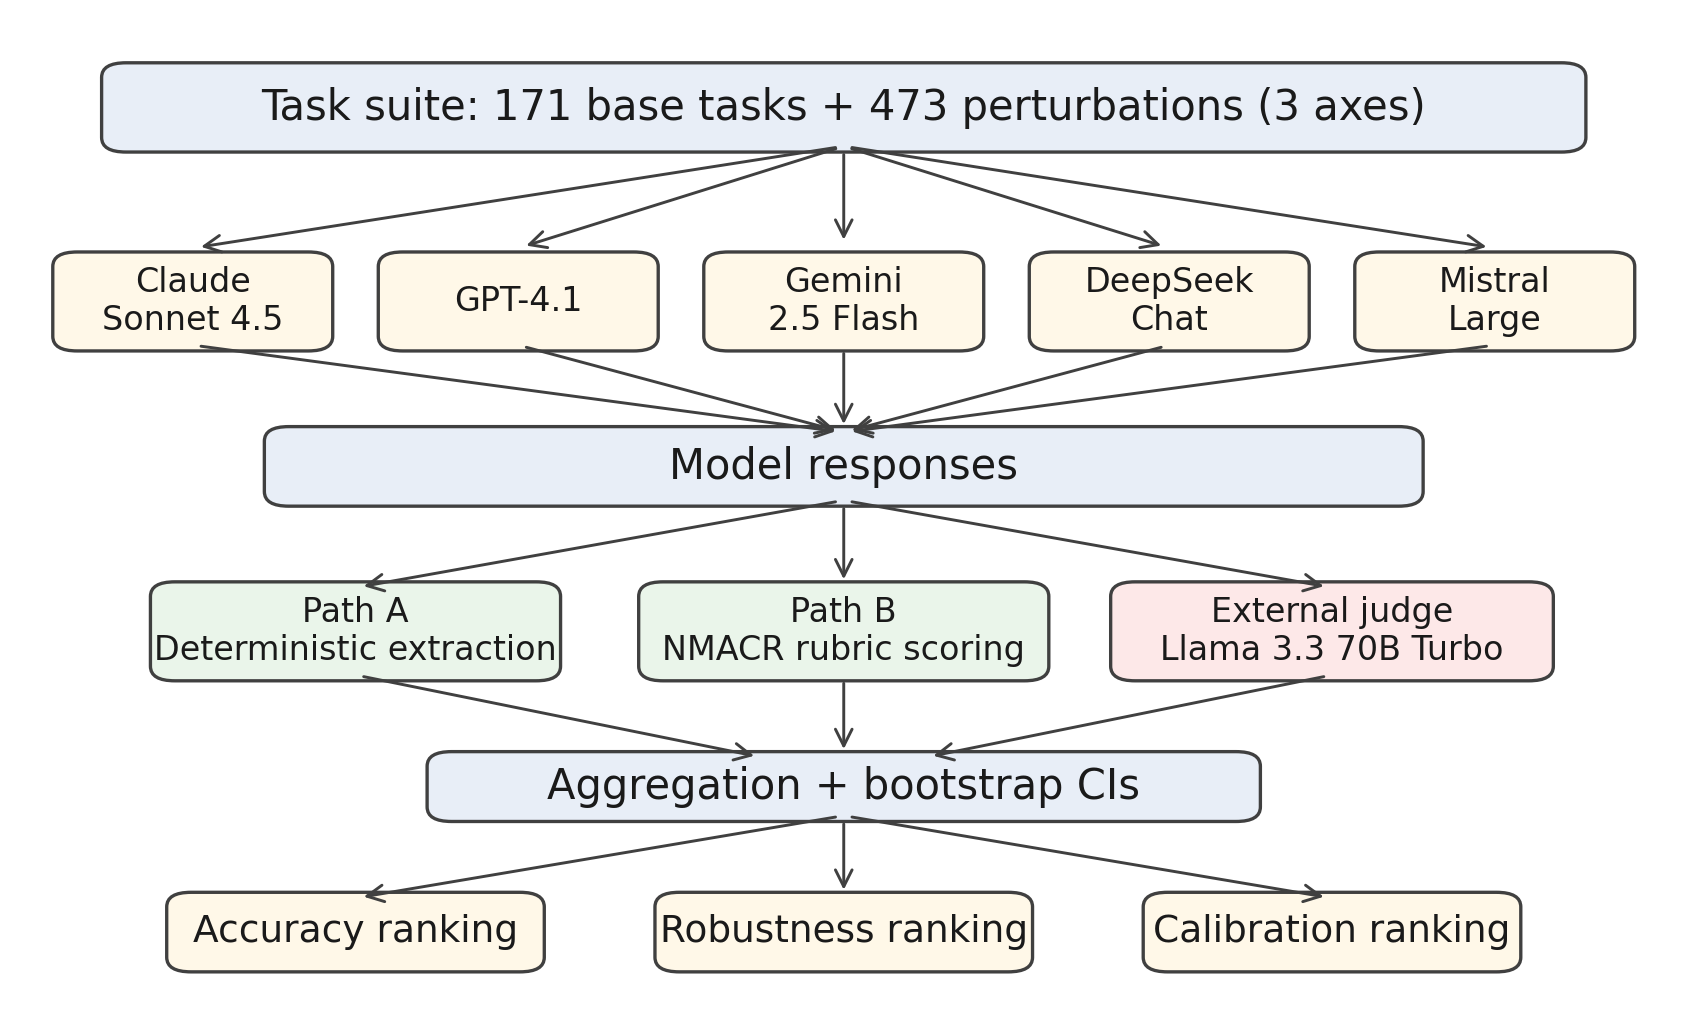
\includegraphics[width=\columnwidth]{figures/pipeline.png}
  \caption{Evaluation pipeline. Each task and its perturbations are
           passed to five frontier LLMs in parallel. Responses are
           scored via three independent paths: deterministic extraction,
           NMACR rubric scoring, and an external Llama 3.3 70B judge
           for assumption-compliance. Aggregated scores yield three
           independent rankings.}
  \label{fig:pipeline}
\end{figure}

\subsection{Perturbation Taxonomy}

Each base task is perturbed along three axes. \emph{Rephrase}
preserves the math and the answer while rewording the prompt.
\emph{Semantic} preserves the math while relocating the problem
to a different real-world framing. \emph{Numerical} changes the
numerical inputs and recomputes the ground-truth answer. The full
set contains 473 records: 75 hand-authored seeds covering 25 base
tasks across all three axes, and 398 LLM-generated perturbations
covering the remaining 146 base tasks, produced by the same Llama
3.3 70B Turbo used as the assumption-compliance judge. Every
LLM-generated perturbation was checked against the ground-truth
solver before inclusion. Mean coverage is 2.77 perturbations per
base task. The numerical axis is skipped for 40 conceptual or
seeded-MC tasks where swapping numbers would invalidate the
ground-truth procedure.

\subsection{Three-Path Scoring}

Each response is scored three ways. \textbf{Path~A} is a
deterministic keyword rubric in the live runner. It extracts the
answer line, compares numeric targets to the ground truth within a
per-task tolerance, and checks required structural and assumption
keywords in the free-form prose. \textbf{Path~B} is a post-hoc
NMACR aggregator. Each task contributes five components in
$[0,1]$: numerical accuracy (N), method structure (M), assumption
compliance (A), confidence calibration (C), and reasoning quality
(R). The combined score is a weighted sum,
\begin{equation}
  S_{\text{NMACR}} = 0.10\,N + 0.20\,M + 0.30\,A + 0.15\,C + 0.25\,R,
  \label{eq:nmacr}
\end{equation}
with weights drawn from the chain-of-thought, calibration, and
assumption-articulation
literature~\cite{wei2022cot,chen2022pot,guo2017calibration,du2025icecream,park2025judge,nagarkar2026canllm,fermieval2025,liu2025matheval}.
A gets the highest weight because assumption articulation is what
Bayesian reasoning is for; N gets the lowest because a correct
number with no derivation does not answer the question. Pass
threshold is $s \geq 0.5$. \textbf{Path~C}, the external judge,
runs on one dimension only. Each (task, response) pair is sent to
Llama 3.3 70B Turbo via the Together AI API with a fixed rubric
prompt asking whether the response explicitly states the
assumptions the task requires. The narrow scope is a direct
response to the holistic-judge failure modes that Feuer et
al.~\cite{judgment2025noise} document.

\subsection{Three-Ranking Framework}

We compute three rank orders from the same response corpus. The
\emph{accuracy ranking} uses the Path~B NMACR pass rate per model
across all 171 base tasks. The \emph{robustness ranking} uses the
perturbation pass-flip rate. Let $\mathrm{pass}(t, m) \in \{0,1\}$
be the binary base pass for task $t$ and model $m$, and
$\overline{\mathrm{pass}}(t, m)$ the mean pass over $t$'s
perturbations $\mathcal{P}(t)$. The model's robustness is
\begin{equation}
  R_m = 1 - \frac{1}{|\mathcal{T}|}\sum_{t \in \mathcal{T}}
        \left| \mathrm{pass}(t, m) - \overline{\mathrm{pass}}(t, m) \right|,
  \label{eq:robustness}
\end{equation}
with $R_m = 1$ for perfect base/perturbation agreement. Bootstrap
CIs use 10{,}000 non-parametric resamples (seed 42). The
\emph{calibration ranking} uses binary-pass Expected Calibration
Error~\cite{guo2017calibration} over $B$ confidence buckets,
\begin{equation}
  \mathrm{ECE} = \sum_{b=1}^{B} \frac{|B_b|}{N}
                 \,\bigl|\,\mathrm{acc}(B_b) - \mathrm{conf}(B_b)\,\bigr|,
  \label{eq:ece}
\end{equation}
where $B_b$ is the set of predictions in bucket $b$,
$\mathrm{acc}(B_b)$ is empirical accuracy within the bucket, and
$\mathrm{conf}(B_b)$ is the bucket's mean confidence. We use
$B = 4$ buckets (low, medium, high, unstated) parsed from the
response's hedging language. The three rankings are not redundant:
a model can be accurate but brittle, accurate and well-calibrated
but brittle, or robust but inaccurate. \S\ref{sec:results} shows
all three of those configurations actually occur in our five-model
sample.

\subsection{Experimental Setup}

\textbf{Models and APIs.} The five LLMs are queried directly over
their HTTP APIs with no vendor SDKs: Claude Sonnet 4.5 (Anthropic
Messages), GPT-4.1 (OpenAI Chat Completions), Gemini 2.5 Flash
(Google Generative Language), DeepSeek-Chat, and Mistral Large.
Decoding settings are the same for every provider. Temperature
is the API default (around 1.0 for the chat endpoints). Max
output is 1024 tokens. Each call has a 60-second timeout and
retries on transient 429 and 5xx responses. The same
Bayesian-statistics system prompt is used for every model.

\textbf{Evaluation pipeline.} Each (task, model) pair produces
one response. Path~A extracts the final answer line and structural
keywords. Path~B aggregates the five NMACR components into a
weighted score. The external Llama 3.3 70B Turbo judge, served by
Together AI's OpenAI-compatible API, scores the response on
assumption-compliance only. Perturbations go through the same three
paths. Single-pass per (task, model) is the default; a small
self-consistency subset (3 samples) is used for the calibration
analysis.

\textbf{Calibration computation.} Equation~\ref{eq:ece} is
computed per model on the full response corpus. Uncertainty is
reported as 95\% percentile bootstrap confidence intervals over
10{,}000 non-parametric resamples of per-run aggregate scores
(seed 42), the same procedure used for the accuracy and robustness
CIs.

\textbf{Reproducibility.} A single shell script drives the full
pipeline: deduplication, scoring, perturbation scoring, judge
invocation, and aggregation. 53 unit tests cover the task
generators and the MCP query interface. Every figure in the paper
is generated by the R analysis pipeline at
\emph{report\_materials/r\_analysis/run\_all.R}; none are
hand-edited.

% --- Section: Experimental Setup ---
% Outline:
%   - Benchmarked models (5 frontier LLMs, all via direct httpx, no SDKs):
%     | family   | model string             | provider                   |
%     | claude   | claude-sonnet-4-5        | api.anthropic.com          |
%     | gemini   | gemini-2.5-flash         | generativelanguage.gapis...|
%     | chatgpt  | gpt-4.1                  | api.openai.com             |
%     | deepseek | deepseek-chat            | api.deepseek.com           |
%     | mistral  | mistral-large-latest     | api.mistral.ai             |
%     Source: llm_runner/model_clients.py (max_tokens 1024, T=60s,
%     retry 3x with provider-specific backoff).
%   - System prompt: ``You are an expert in Bayesian statistics and
%     probability theory. Solve problems step by step, showing all working.
%     Always end your response with your final answer on its own line in
%     the format: ANSWER: <value1>, <value2>, ...''
%   - Scoring (two paths must remain weight-aligned):
%     - Path A: live runner (llm_runner/response_parser.py:full_score),
%       weights N=M=A=C=R=0.20. CONCEPTUAL = 1.0 * rubric_score; tasks
%       with numeric+rubric = 0.6 numeric + 0.4 rubric.
%     - Path B: post-hoc (evaluation/metrics.py:score_all_models) on
%       TaskRun dataclasses, identical weights.
%     - Pass threshold: final_score >= 0.5.
%   - Calibration / ECE computation:
%     - Source: scripts/calibration_analysis.py and
%       experiments/results_v2/calibration.json (per-model bins,
%       reliability diagrams).
%     - extract_confidence() from raw text; overconfident-on-wrong
%       penalized 1.5x, underconfident-on-right 0.8x (Path A).
%   - Sample-size accounting:
%     - 171 base * 5 models = 855 base runs.
%     - 473 perturbations * 5 models = 2365 perturbation runs.
%     - All 855 + 2365 = 3220 LLM responses scored by keyword rubric;
%       judge-scored subset n=143 failure pool for taxonomy. Source:
%       experiments/results_v2/{robustness_v2,calibration,
%       error_taxonomy_v2,perturbation_runs}.json[l].
% TODO: prose draft

\section{Experimental Setup}
\label{sec:setup}
% placeholder

% --- Section: Results ---
% Outline:
%   - Three rankings overview (figure: three_rankings.png from
%     report_materials/figures/, regenerated by
%     scripts/three_rankings_figure.py):
%     - Accuracy ranking from experiments/results_v1/results.json
%       (model_aggregates).
%     - Robustness ranking (perturbation pass-flip rate) from
%       experiments/results_v2/robustness_v2.json + bootstrap_ci.json.
%     - Calibration ranking (ECE) from
%       experiments/results_v2/calibration.json + per_dim_calibration.json.
%   - Headline: top-2 swap. Claude leads accuracy; ChatGPT leads
%     calibration. Discuss why this matters numerically.
%   - Assumption-compliance gap: 51.5% of responses fail to state required
%     assumptions (judge dimension). Source:
%     experiments/results_v2/error_taxonomy_v2.json l1_totals
%     ASSUMPTION_VIOLATION = 67/143; report_materials/figures/
%     a3_failure_heatmap.png; failure_taxonomy_stacked.png.
%   - Judge agreement: keyword rubric vs external judge Spearman rho =
%     0.59 (Krippendorff alpha and pairwise from
%     experiments/results_v2/krippendorff_agreement.json,
%     keyword_vs_judge_agreement.json). Figure:
%     report_materials/figures/agreement_metrics_comparison.png.
%   - Perturbation breakdown by axis (rephrase / numerical / semantic).
%     Figure: a4_robustness_by_perttype.png and
%     a4b_per_dim_robustness.png.
%   - Per-dimension calibration. Figure: a5b_per_dim_calibration.png and
%     calibration_reliability.png.
%   - Failure taxonomy. Figure: error_taxonomy_hierarchical.png; pull
%     L1 / L2 totals from error_taxonomy_v2.json.
% TODO: prose draft + figure inserts (\includegraphics from figures/)

\section{Results}
\label{sec:results}
% placeholder

% --- Section: Analysis and Validation ---

\section{Analysis and Validation}
\label{sec:discussion}

\textbf{What the three-ranking divergence means.} The three metrics
are not the same axis under different names. Each has deployment
consequences the others do not capture. Accuracy is the natural
signal for one-shot question answering. For pipelines that
paraphrase prompts or swap inputs (automated tutoring, agentic
workflows), robustness matters more: picking by accuracy alone for
paraphrase-heavy pipelines can be exactly wrong. For systems that
gate decisions on expressed confidence (triage tools, ensemble
selectors), calibration matters, and DeepSeek's ECE of $0.198$
rules it out regardless of accuracy.

\textbf{Reasoning versus pattern matching.} The keyword-vs-judge
gap on assumption-compliance is the clearest evidence for the paper's
title. On the combined base-and-perturbation pool ($n = 2{,}850$),
$20.7\%$ of responses pass-flip between the two scorers. On the
$n=750$ base-only pool, the judge passes $55.7\%$ versus the
keyword rubric's $71.1\%$, a $15.4$-point gap that indicates the
direction: surface-form scoring overcounts substantive
articulation~\cite{du2025icecream}. The calibration analysis
(Table~\ref{tab:calibration-paired}) shows the same shape:
verbalized confidence places Claude and GPT-4.1 in the
well-calibrated tier (ECE $\approx 0.033$), while self-consistency
on three reruns at $T = 0.7$ puts every model past the
$\text{ECE} = 0.6$ ``severe overconfidence'' threshold.

\textbf{Broader implications.} The multi-axis ranking is cheap to
add: the same response corpus feeds robustness once perturbations
exist and calibration once confidence is parsed. Single-number
leaderboards should be reported alongside the multi-axis view, not
in place of it.

\subsection{Decomposing the Divergence: Four Orthogonal Signals}
\label{sec:decomposition-synthesis}

The three-ranking divergence is one coarse-grained view. \S
\ref{sec:extended-diagnostics} decomposes it into four orthogonal
diagnostic signals.
\textit{(i) Model-specific over-credit}
(\S\ref{sec:per-model-disagreement}): Mistral $12.11\times$ and
Claude $7.84\times$ keyword-judge asymmetry, vs GPT-4.1
$2.58\times$ --- surface-token credit is not uniform across the
benchmarked LLMs.
\textit{(ii) Task-specific failure concentration}
(\S\ref{sec:failure-by-task-type}): all 143 L1 failures fall in
Phase~1, with the Bayesian-regression families
(\texttt{REGRESSION}+\texttt{BAYES\_REG}) absorbing $35\%$;
failures hit all five models uniformly within each task type, so
the over-credit problem and the task-difficulty problem are
independent.
\textit{(iii) Axis-specific robustness}
(\S\ref{sec:per-axis-robustness}): rephrasing ($R=0.966$) hurts
more than numerical perturbation ($R=0.978$), with model variance
$3.66\times$ axis variance --- the robustness ranking is a real
model property, but GPT-4.1's $0.9996$ is a near-cancellation of a
rephrasing drop and gains on the other two axes.
\textit{(iv) Phase-specific rank flips}
(\S\ref{sec:per-phase-performance}): Mistral climbs from 5th on
Phase~1 to 2nd on Phase~2 ($+3$ positions), driven by the
assumption-compliance bar dropping on procedural prompts where the
rubric expects no explicit prior or likelihood statement.

A model can be top-ranked on one signal and bottom-ranked on
another --- the four are not a single latent factor under different
names. Mistral concretely illustrates this: 5th on Phase~1 NMACR
but 2nd on Phase~2; the strongest pattern-matcher per
\S\ref{sec:per-model-disagreement} but the second-most-robust per
\S\ref{sec:per-axis-robustness}. Pattern matching as a strategy is
robust --- surface tokens propagate cleanly through paraphrase and
number-swap --- and pays off on tasks where the rubric accepts
surface-correct procedural prose. It collapses only on tasks with
substantive assumption-articulation requirements that the judge
actually checks (Phase~1 conjugate derivations, specifically
Bayesian linear regression).

A single-metric leaderboard does not just collapse the
three-ranking divergence from \S\ref{sec:results}: it collapses
four orthogonal diagnostic axes. The title question admits a more
specific answer than the headline three-ranking captures: pattern
matching is real, model-specific, axis-stable, and rewarded by
procedural task structure. A reader picking a model for Bayesian
work should inspect all four \S\ref{sec:extended-diagnostics}
columns alongside the headline accuracy and calibration numbers ---
the aggregate scoreboard hides which model is genuinely reasoning
and which is fluent at the surface.

% --- Section: Threats to Validity ---
% Outline:
%   - Judge bias risk:
%     - External judge (Llama 3.3 70B Turbo) is out-of-family vs the 5
%       benchmarked LLMs, eliminating self-preference. But Llama is still
%       an LLM and may share systematic biases. Mitigation: keyword-rubric
%       cross-check (rho=0.59 with judge); top_disagreements_assumption.json
%       inspected manually. Cite park2025judge, judgment2025noise.
%     - Source: llm-stats-vault/90-archive/audit/limitations_disclosures.md.
%   - Task-coverage limits:
%     - 171 tasks span 31 + 7 = 38 task types; not exhaustive of Bayesian /
%       inferential statistics. MCMC tasks are advanced-only (35); Phase 1
%       conjugate models dominate. Source: bayesian_scope.md.
%   - Perturbation construct validity:
%     - LLM-generated perturbations (398 of 473) inherit any framing biases
%     of the generator (Llama 3.3 70B). Hand-authored seeds (75) provide
%     a control. Per-base coverage: 40 bases have only 2 perturbations
%     (numerical mutation skipped where infeasible).
%   - Sample-size caveats:
%     - 855 base runs + 2365 perturbation runs scored by keyword rubric;
%       n=143 judge-scored failures for the L1/L2 taxonomy. Per-cell counts
%       (model x task type x perturbation type) get small (sometimes < 5).
%       Bootstrap CIs (experiments/results_v2/bootstrap_ci.json) report
%       uncertainty; rank-shift sensitivity in
%       experiments/results_v2/tolerance_sensitivity.json.
%   - Scoring-weight choice (N=M=A=C=R=0.20):
%     - Equal-weight choice is a methodology decision; rankings could
%       shift under alternative weightings. Cite NMACR robustness analysis
%       in experiments/results_v2/nmacr_scores_v2.jsonl and
%       methodology_continuity.md.
%   - API drift: model versions are pinned (e.g. claude-sonnet-4-5,
%     gpt-4.1, mistral-large-latest) but ``-latest'' tags are not
%     reproducible long-term. Run timestamps preserved in runs.jsonl.
% TODO: prose draft

\section{Threats to Validity}
\label{sec:threats}
% placeholder

% --- Section: Conclusion ---
% Drafted Phase 6 Checkpoint C. Merged with prior §07 threats-to-validity
% and future-work content per A.5 structure migration.
% Target: ~400 words (200 conclusion + 200 threats/limitations).

\section{Discussion and Conclusion}
\label{sec:conclusion}

We benchmarked five frontier LLMs on 171 Bayesian and inferential
statistical tasks with 473 perturbations, scored by a deterministic
keyword rubric, an NMACR aggregator with literature-derived weights,
and an out-of-family Llama 3.3 70B Turbo judge constrained to
assumption-compliance. The five models produce three different rank
orders depending on the axis. The model with the lowest base
accuracy (GPT-4.1, $0.621$) is the most robust to perturbation
($0.9996$); the model that leads accuracy ($0.683$) and binary-pass
calibration (ECE $0.0334$) drops to fourth on robustness ($0.9565$).
Independently, $44.3\%$ of responses do not articulate the
assumptions the derivation requires, and the keyword rubric
overcounts assumption articulation by $15.4$ percentage points
relative to the judge. A single number is the wrong instrument for
statistical-reasoning evaluation; the right ranking depends on the
property being measured.

\textbf{Threats to validity.} The Llama 3.3 70B Turbo judge can
carry systematic biases from its training. We constrain it to one
dimension rather than asking for a holistic preference signal, and
we validate it against the keyword rubric (Spearman $\rho = 0.602$
on assumption-compliance). Krippendorff's $\alpha$ on the three
judged dimensions sits in the ``questionable'' range. That reflects
genuine ambiguity in scoring free-form Bayesian reasoning, not
instrument failure, and we report it as honest disclosure. The
three-ranking divergence is a within-model cross-metric finding
and does not depend on inter-rater agreement. Task coverage is
broad for Bayesian and inferential reasoning but is not
representative of statistical reasoning generally; causal inference
and experimental design are out of scope. Mean perturbation count
is $2.77$ per base task, and ECE estimates use 10{,}000-sample
bootstrap CIs that carry the uncertainty through. Model versions
are May 2026 snapshots; the inversion patterns may not replicate
as APIs evolve.

\textbf{Future work.} Three extensions follow. First, broaden the
task suite into causal inference, experimental design, and
frequentist hypothesis testing, to see whether the three-axis
divergence generalizes outside Bayesian reasoning. Second,
replicate with a second out-of-family judge to bound judge-bias
variance; cross-judge agreement on assumption-compliance would
also act as an upper bound on inter-rater reliability for the
dimension. Third, treat the GPT-4.1 inversion as a hypothesis
about training-data composition and decoding choices, and run
controlled experiments at the provider level that isolate the
relevant factors.


\bibliographystyle{IEEEtran}
\bibliography{bib/refs}

\end{document}
